\chapter{Deep Learning}

	En este capítulo nos centramos en las técnicas implementadas a lo largo de la memoria, técnicas de \textit{Deep Learning}. Los diferentes modelos que implementaremos se basan en redes neuronales, por lo que dedicaremos la primera sección de este capítulo a hablar sobre redes neuronales prealimentadas. También se tratarán las características generales de las redes neuronales que nos servirán como base introductoria de los modelos desarrollados.
	
	A continuación, desarrollaremos en profundidad los modelos implementados: redes neuronales convolucionales y redes neuronales recursivas (LSTM). 
	
	%Por último, daremos una justificación teórica del comportamiento de estos modelos en el problema concreto que estamos tratando.

\section{Redes Neuronales Prealimentadas}

Las \textbf{redes neuronales} son el ejemplo más típico de modelos de \textit{Deep Learning}. El objetivo de esta clase de algoritmos es aproximar una función $f^*$. Por ejemplo, para un clasificador $y = f^*(x)$ que asocia a cada entrada $x$ una categoría $y$. Así, una red neuronal prealimentada define una asociación $y = f(x; \theta)$ y aprende los valores de los parámetros $\theta$ que ofrecen la mejor aproximación de la función.

Esta clase de modelos se llaman \textbf{prealimentados} porque la información fluye a través de la función siendo evaluados desde $x$, mediante los cálculos intermedios usados para definir $f$ y finalmente hasta la salida $y$. Por tanto, nunca se forman ciclos entre las conexiones de las unidades, la información se evalúa siempre hacia delante a través de las diferentes capas intermedias. No existe ningún tipo de retroalimentación en las que la salida de alguna capa de la red vuelva a ser entrada del modelo. 

Las redes neuronales son llamadas \textbf{redes} pues se definen mediante la composición de diferentes funciones. Este modelo de sucesivas composiciones se puede ver como un grafo dirigido acícilo.  

El número de capas que tenga la red definen la \textbf{profundidad} del modelo. Las capas se van nombrando de forma sucesiva siendo la primera la primera capa o \textit{capa de entrada}, \textit{segunda capa}, y así sucesivamente hasta la capa final denominada \textit{capa de salida}. El objetivo del modelo es conducir la función de entrada $f(x)$ para que se ajuste a $f^*(x)$. 

Este tipo de algoritmos están inspirados en la neurociencia, en concreto en las neuronas de los seres vivos. Cada capa del modelo está formado por un número de unidades. El número de unidades en cada capa define la \textbf{anchura} del modelo. Cada una de estas unidades que actúa de forma paralela, representa una neurona que recibe información de otras unidades (neuronas) y calcula su propio valor de activación. 

\begin{figure}[h!]
	\centering
	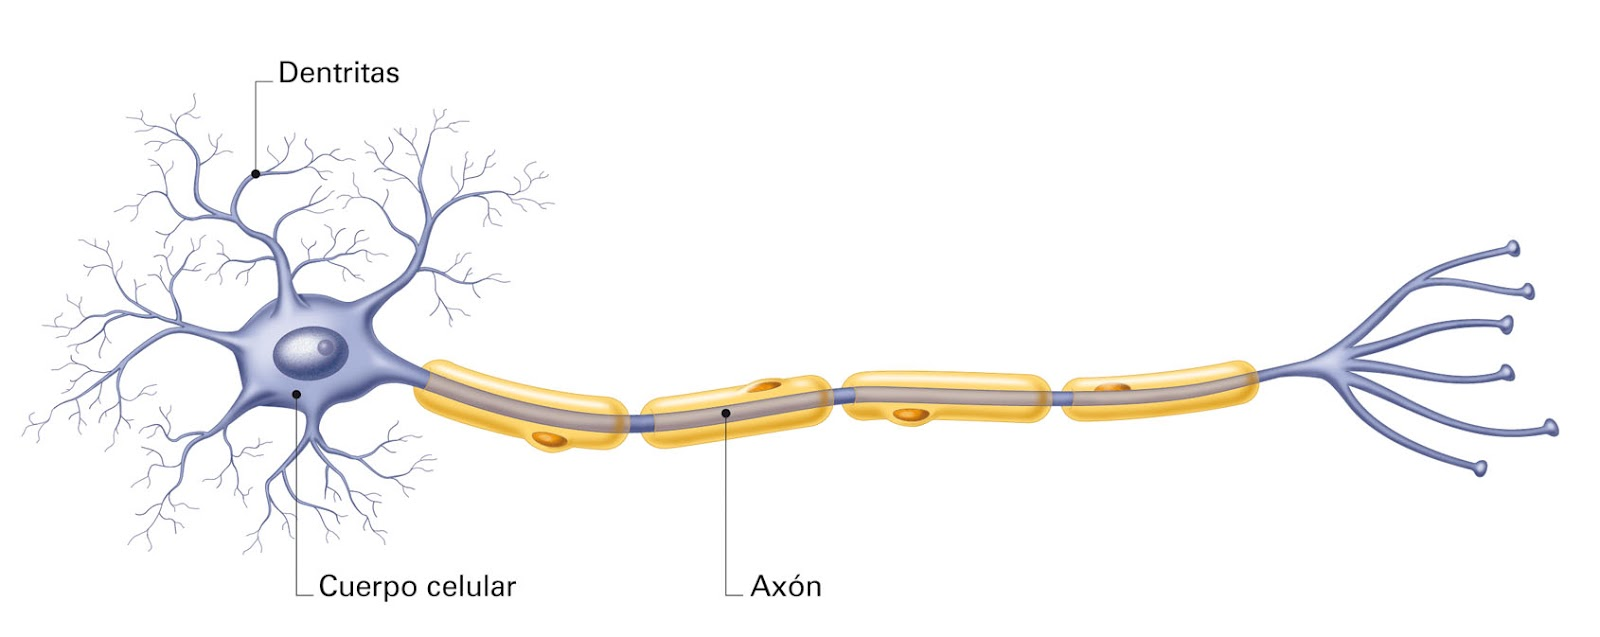
\includegraphics[width=0.7\linewidth]{imagenes/Neurona}
	\caption{Representación de una neurona biológica.}
	\label{fig:neurona}
\end{figure}


El símil con las neuronas de los seres vivos es que estas se componen de dentritas que se encargan de recoger los estímulos de otras neuronas (entradas), un núcleo para su almacenamiento (activación) y un axón con terminales que le permiten transmitir los impulsos a otras neuronas (salidas).

\begin{figure}[h!]
\centering
\begin{tikzpicture}[
init/.style={
	draw,
	circle,
	inner sep=2pt,
	join = by -latex
},
squa/.style={
	draw,
	inner sep=2pt,
	join = by -latex
},
start chain=2,node distance=13mm
]
\node[on chain=2, init] 
(x2) {$x_2$};
\node[on chain=2,join=by o-latex] 
{$w_2$};
\node[on chain=2,init ,label={[label distance=0.75cm]below:Activación}] (sigma)
{$ g(w^tx + b)$};
\node[on chain=2, init ,label={[label distance=1.5cm]below:Salida}](y)
{$y$};
\begin{scope}[start chain=1]
\node[on chain=1, init] at (0,1.5cm) 
(x1) {$x_1$};
\node[on chain=1,join=by o-latex] 
(w1) {$w_1$};
\end{scope}
\begin{scope}[start chain=3]
\node[on chain=3, init ,label=below:Entradas] at (0,-1.5cm) 
(x3) {$x_3$};
\node[on chain=3,join=by o-latex,label=below:Pesos] 
(w3) {$w_3$};
\end{scope}

\draw[-latex] (w1) -- (sigma);
\draw[-latex] (w3) -- (sigma);
\draw[-latex](sigma) -- (y);

\end{tikzpicture}
\caption{Representación de una neurona artificial de 3 entradas con función de activación g.}
\label{fig:neuron_articial}
\end{figure}

La neurona artificial se define como en la Figura \ref{fig:neuron_articial}, donde identificamos una neurona biológica con una función $f: \mathbb{R}^n \rightarrow \mathbb{R}$ donde $n$ es el número de unidades en la capa anterior (entradas).

En conclusión, una red neuronal artifical estaría formada por un número arbitrario de capas y un número arbitrario de unidades (neuronas artificiales) en cada capa. 

\begin{figure}[h!]
	\centering
	\begin{tikzpicture}[
	init/.style={
		draw,
		circle,
		font = \Large,
		inner sep=2pt,
		join = by -latex
	},
	squa/.style={
		draw,
		inner sep=2pt,
		join = by -latex
	},
	start chain=2,node distance=13mm
	]
	\node[on chain=2, init] 
	(x2) {$x_2$};
	

	\begin{scope}[start chain=1]
		\node[on chain=1, init] at (0,1.5cm) 
		(x1) {$x_1$};
	\end{scope}
	
	\begin{scope}[start chain=3]
		\node[on chain=3, init ,label={[label distance=2cm]below:Entradas}] at (0,-1.5cm) 
		(x3) {$x_3$};
	\end{scope}
	
	\begin{scope}[start chain=4]
	\node[on chain=3, init] at (1.5,3cm) 
	(h1) {$h_1$};
	\end{scope}
	
	\begin{scope}[start chain=5]
	\node[on chain=3, init] at (1.5, 1cm) 
	(h2) {$h_2$};
	\end{scope}
	
	\begin{scope}[start chain=6]
	\node[on chain=3, init] at (1.5,-1cm) 
	(h3) {$h_3$};
	\end{scope}
	
	\begin{scope}[start chain=7]
	\node[on chain=3, init,label={[label distance=0.5cm]below:Capa oculta}] at (1.5,-3cm) 
	(h4) {$h_4$};
	\end{scope}
	
	\begin{scope}[start chain=8]
		\node[on chain=8,init, label= {[label distance=3.6cm]below:Salida}] at (7,0 cm) (sigma)
	{y};
	\end{scope}
	
	
	
	\draw[-latex] (x1) -- (h1);
	\draw[-latex] (x1) -- (h2);
	\draw[-latex] (x1) -- (h3);
	\draw[-latex] (x1) -- (h4);
	\draw[-latex] (x2) -- (h1);
	\draw[-latex] (x2) -- (h2);
	\draw[-latex] (x2) -- (h3);
	\draw[-latex] (x2) -- (h4);
	\draw[-latex] (x3) -- (h1);
	\draw[-latex] (x3) -- (h2);
	\draw[-latex] (x3) -- (h3);
	\draw[-latex] (x3) -- (h4);

	\draw[-latex](h1) -- (sigma);
	\draw[-latex](h2) -- (sigma);
	\draw[-latex](h3) -- (sigma);
	\draw[-latex](h4) -- (sigma);
	
	\end{tikzpicture}
	\caption{Representación de una neurona artificial de 3 entradas con función de activación g.}
	\label{fig:rrnn_artifical}
\end{figure}

  
Observamos en la Figura \ref{fig:rrnn_artifical} un ejemplo simplificado de una red neuronal con tres capas: capa de entrada, una capa oculta y capa de salida. La capa de entrada tiene tres unidades, la oculta cuatro y la de salida una.

Una forma de entender las redes neuronales prealimentadas es conocer las limitaciones de los modelos lineales y considerar cómo superarlas. El éxito de los modelos lineales como la regresión logística o lineal radica en su eficiencia y fiabilidad. Sin embargo, no se puede  ignorar el  inconveniente de que están limitados a funciones lineales, por tanto no contemplan las posibles relaciones entre dos variables de entrada.

Para extender estos modelos de forma que representen funciones no lineales de $x$, podemos considerar un modelo lineal sobre una transformación de la entrada $\phi(x)$ donde $\phi$ es una transformación no lineal. El problema se traduce, entonces, en encontrar qué transformación no lineal $\phi$ aplicar a la entrada $x$:

\begin{itemize}
	\item La primera opción sería estudiar manualmente qué función se ajusta más al problema concreto, lo que conllevaría un alto conocimiento del problema.
	\item Otra opción sería utilizar una función genérica $\phi$ de alta dimensionalidad para que siempre tenga la suficiente capacidad de adaptarse al conjunto de entrenamiento, lo cual no proporciona una buena generalización en el conjunto de test.
	\item El enfoque que aporta el \textit{deep learning} es aprender $\phi$ en un conjunto de funciones parametrizadas. Así, tenemos el modelo 
	$$y = f(x; \theta, w) = \phi(x; \theta)^T w$$ 
	
	donde $\theta$ es un conjunto de parámetros utilizado para aprender $\phi$ de entre la clase de funciones consideradas. 
\end{itemize}

	Este modelo nos aporta una gran flexibilidad pues la elección de la función de transformación depende del conjunto de funciones que estemos considerando. Además, al igual que en los modelos lineales deberemos predefinir ciertos aspectos de diseño: optimizador, función de coste y forma de las unidades de salida. Las redes neuronales prealimentadas introducen el concepto de capa oculta, por lo que tendremos que elegir también las funciones de activación que se utilizarán para calcular la salida de cada una de estas capas. También será necesario definir la arquitectura de la red, definiendo cuántas capas añadir y cuántas unidades tendrá cada una.  
	
	A continuación estudiaremos algunas de las funciones comentadas.
	
	\subsection{Función de coste}
	
	La principal diferencia entre los algoritmos lineales y las redes neuronales es la ya comentada no linealidad. Esta característica hace especialmente interesante considerar funciones de coste no convexas en este tipo de modelos. 
	
	Aunque en algunos casos podemos definir la función de coste como un estadístico de $y$ condicionado a $x$. En la mayoría de los diseños, el modelo paramétrico definido define una distribución de probabilidad $ p(y | x ; \theta)$ y podemos aplicar el principio de máxima verosimilitud comentado en la Sección \ref{prob}. Esto significa que usamos la entropía cruzada entre los datos de entrenamiento y las predicciones del modelo como función de coste:
	
	$$
		J(\theta) = - \mathbb{E}_{x,y \sim \hat{p}_{data}} \log p_{model}(y | x)
	$$
	
	La ventaja de esta función de coste es que queda determinada en función de $p_{model}(y|x)$ ahorrándonos el trabajo de definir una función de coste propia para cada problema. Además, un tema recurrente en el diseño de redes neuronales es que el gradiente de la función de coste debe ser grande para evitar que el valor del gradiente vaya rápidamente a cero y nuestra función de coste cumple este requisito.
	
	
	\subsection{Unidades de salida}
	
	La elección de la función de coste está estrechamente relacinada con la elección de la unidad de salida. La mayoría de las veces simlpemente utilizamos la entropía cruzada de la distribución de los datos y de la distribución del modelo.
	
	Aunque en esta sección nos centremos en unidades de salida, estas funciones pueden ser	utilizadas en las capas ocultas también. Para unificar la  notación supondremos que la red neuronal produce una salida de las capas ocultas definida por el vector de características $h = f(x; \theta)$. 
	
	Aunque existen muchas posibiildades, las principales unidades de salida son de los siguientes tipos:
	
	\subsubsection{Unidades lineales}
		
		Un tipo de unidad de salida está basada en una transformación lineal. Esto es, dado el vector de características $h$, la capa produce como salida el vector 
		
		$$
			\hat{y} = W^Th + b
		$$ 
		
		El uso principal de este tipo de unidades de salida es producir la media de una distribución condicional normal:
		
		$$
			p(y | x) = \mathcal{N}(y; \hat{y}, I)
		$$ 
		
		Para esta probabilidad condicionada concreta, calcular la entropía cruzada (log-verosimilitud negativa) es equivalente a minimizar usando el error cuadrático medio.
		
	\subsubsection{Unidades sigmoidales}
	
		Este tipo de unidades se utilizan para tareas que requieren la predicción de una variable binaria $y$. La probabilidad condicionada aplicada en la técnica de máxima verosimilitud en este caso se correspondería con la definición de una distribución de Bernouilli sobre $y$ condicionada a $x$. Esta distribución se define con un número en el intervalo $[0,1]$ determinado por la probabilidad  $P(y = 1 | x)$. 
		
		Para cumplir la restricción de permanecer en el intervalo $[0,1]$ podríamos considerar la función de probabilidad
		
		$$
			P(y = 1|x) = \max\{0, \min\{ 1, w^Th + b\}\}
		$$
		
		Sin embargo, esto tiene un problemapues cada vez que el valor de la expresión $w^Th + b$ quedara fuera del intervalo, el gradiente valdría 0, lo cual supondría un mal funcionamiento del método.
		
		Para asegurar un buen funcionamiento del método, asegurándonos de que el gradiente no es muy cercano a cero se utiliza un enfoque diferente. Consiste en utilizar una salida sigmoidal combinada con el criterio de máxima verosimilitud.
		
		Así, a salida de una unidad de salida sigmoidal estaría definida por 
		
		$$
			\hat{y} = \sigma (w^Th + b) = \frac{1}{1 + e^{-(w^Th + b)}}
		$$
		
		Podemos ver esta salida como una unidad que tiene dos componentes:
		\begin{enumerate}
			\item En primer lugar se aplica una capa lineal para calcular $z = w^Th + b$
			\item En segundo lugar se aplica una \textbf{función de activación sigmoidal} para convertir $z$ en una probabilidad.
		\end{enumerate}
		
		Para construir la distribución de probabilidad sobre $y$ podemos partir de una distribución de probabilidad $\tilde{P}(y)$ no normalizada (no suma 1). A partir de aqui, podemos obtener una distribución de probabilidad dividiendo entre la constante adecuada y que $y \in \{0,1\}$, obteniendo:
 		
 		$$
	 		log \tilde{P}(y) = yz,
	 	$$
	 	$$
		 	\tilde{P}(y) = e^{yz},
	 	$$
	 	$$
	 		P(y) = \frac{e^{yz}}{e^{yz} + e^{(1-y)z}} = \frac{1}{1 + \frac{e^z}{e^{2yz}}} = \frac{1}{1 + e^{(1-2y)z}},
	 	$$
	 	$$
	 		P(y) = \sigma((2y-1)z) 		
 		$$
 		
 		Hemos obtenido que la función de distribución sobre $y$ es una Bernouilli determinada por la transformación logística de $z$.
 		
 		Susituyendo esta función de probabilidad en la fórmula de la entropía cruzada obtenemos:
 		
 		$$
	 		J(\theta) = -\log P(y|x) = -\log \sigma((2y-1)z)  		
 		$$
 		
 		que está bien definida pues $\sigma$ está definida en $(0,1)$ abierto por lo que su logaritmo es finito y bien definido.
 		
 		\begin{figure}[h!]
 			\centering
 			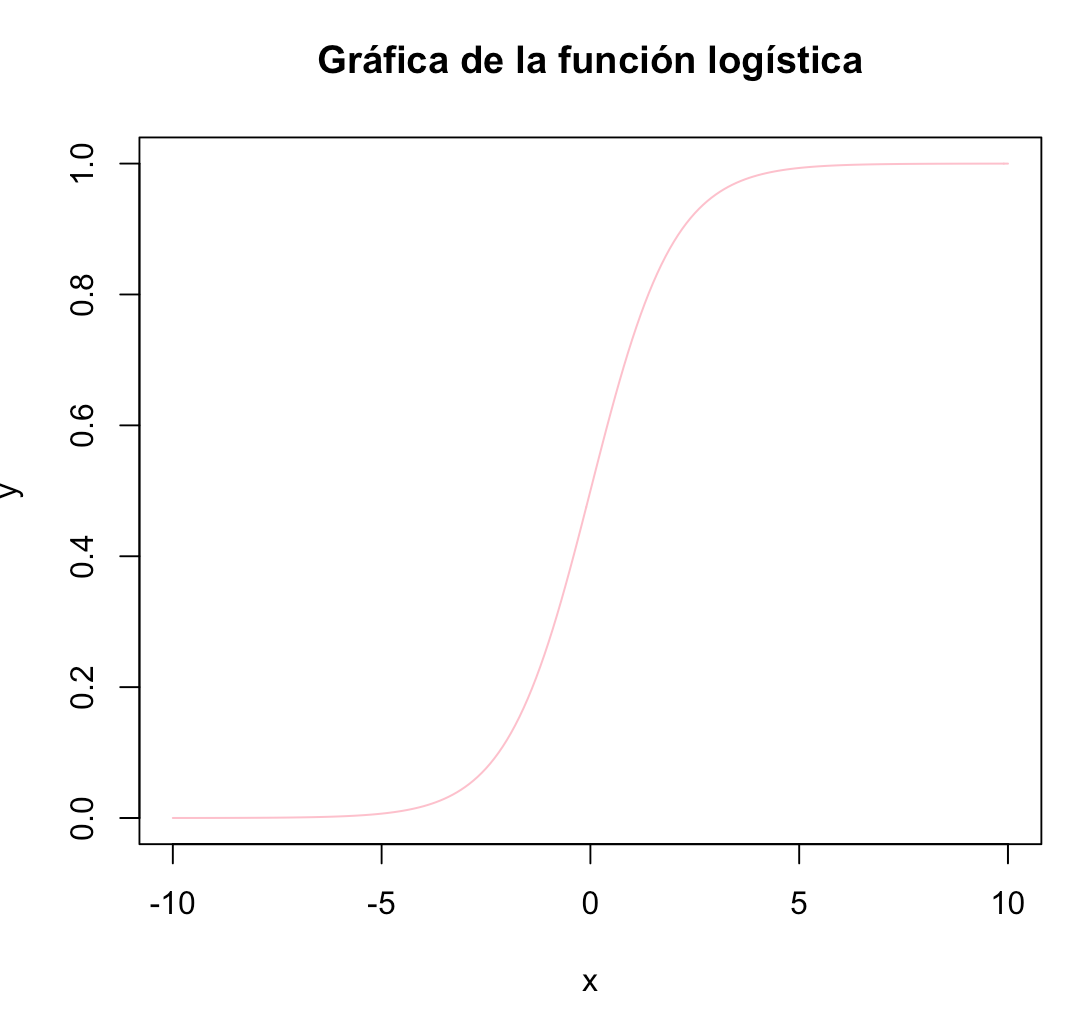
\includegraphics[width=0.7\linewidth]{imagenes/log}
 			\caption{Gráfica de la función logística. Toma valores en (0,1)}
 			\label{fig:log}
 		\end{figure}
 		 
		
	\subsubsection{Unidades con activación softmax}
		
		Cada vez que queramos representar una distribución de probabilidad sobre una variable discreta que toma $n$ valores diferentes, usaremos la\textbf{función de activación \textit{softmax}}. Podemos ver esta función como una generalalización de una función sigmoidal.
		
		En la práctica, este tipo de unidades de salida son muy utilizadas en los algoritmos de clasificación, para representar la distribución de probabilidad de pertenecer a las diferentes $n$ clases. De forma extraordinaria también se pueden utilizar en las capas intermedias del modelo si queremos que el modelo elija entre una de las $n$ diferentes opciones en alguna variable interna.
		
		Para generalizar el caso anterior a una variable discretade $n$ valores, necesitamos producir un vector $\hat{y}$ con $\hat{y}_i=P(y=i|x)$. En este caso se añade a la condición de que cada $\hat{y}_i$ esté entre 0 y 1 que la suma del vector sea 1 para que represente una distribución de probabilidad. 
		
		Utilizando la misma filosofía que en el caso anterior definimos una probabilidad logarítmica no normalizada
		
		$$
			z = W^Th +b
		$$
		
		donde $z_i = \log \tilde{P}(y = i | x)$. 
		
		Pasando a exponencial y normalizando obtenemos la función \textit{softmax}
		
		$$
			softmax(z)_i = \frac{e^{z_i}}{\sum_{j} e^{z_j}}
		$$
		
		De nuevo, la función de coste se obtendría sustituyendo el valor en la función de entropía cruzada.

	\subsection{Unidades ocultas}
	
	Aunque cualquiera de las funciones de activación comentadas en la sección anterior se pueden aplicar en las unidades de una capa oculta, existen otras más adecuadas para ello. De hecho, el diseño de las unidades ocultas es un campo de investigación muy activo. A lo largo de esta sección desarrollaremos algunas de las más comunes.
	
	\subsubsection{Unidades lineales rectificadas (ReLu) y generalizaciones}
	 
	 Las unidades lineales rectificadas usan como función de activación
	 
	 $$
		 g(z) = \max\{0,z\}
	 $$
	 
	 Estas unidades son fácil de optimizar dado que son muy similares a las unidades lineales. La única diferencia radica en que la unidad lineal rectificada toma el valor 0 en la mitad del su dominio. Observamos la gráfica en la Figura \ref{fig:relu}.
	 
	 \begin{figure}[h!]
	 	\centering
	 	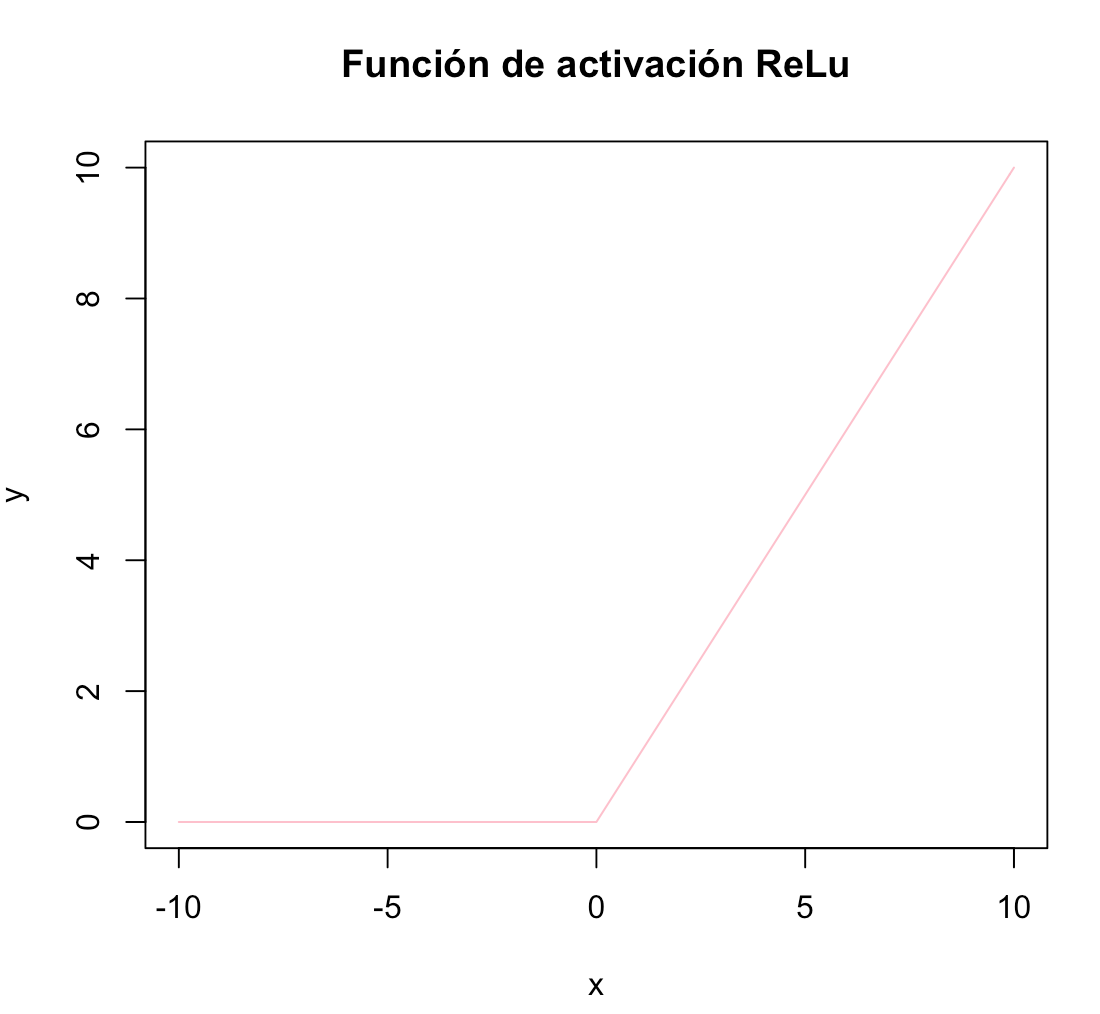
\includegraphics[width=0.7\linewidth]{imagenes/relu}
	 	\caption{Gráfico de la función de activación de las unidades lineales rectificadas.}
	 	\label{fig:relu}
	 \end{figure}
 
	 Existen muchas modificaciones de las unidades lineales rectificadas. Una desventaja de este tipo de unidades es que no pueden aprender usando métodos basados en gradiente en los ejemplos cuya activación sea 0. Muchas de las 8generalizaciones intentan solventar este problema. Definen $h_i = g(z, \alpha)_i = \max(0, z_i) + \alpha_i \min(0, z_i)$ y varían en el valor de las $\alpha_i$:
	 
	 \begin{enumerate}
		 \item \textbf{Rectificación valor absoluto}: fija $\alpha_i = -1$ para obtener $g(z) = |z|$.
		 \item \textbf{\textit{Leaky} ReLu: } fijan $\alpha_i$ a un valor pequeño por ejemplo $0.01$.
		 \item \textbf{ReLu paramétrica: } utiliza valores de $\alpha_i$ no fijos, paramétricos.
	 
	\end{enumerate}
	 
	 
	 \subsubsection{Sigmoidal y tangente hiperbólica}
	
	Antes de la introducción de las unidades lineales rectificadas, la mayoría de las redes neuronales usaban la función sigmoidal de activación 
	
	$$
		g(z) = \sigma(z) = \frac{1}{1 + e^-z}
	$$
	
	cuya gráfica podemos observar en la Figura \ref{fig:log} o la tangente hiperbólica como función de activación
	
	$$
		g(z) = \tanh(z)
	$$
	
	cuya gráfica es 
	
	\begin{figure}[h!]
		\centering
		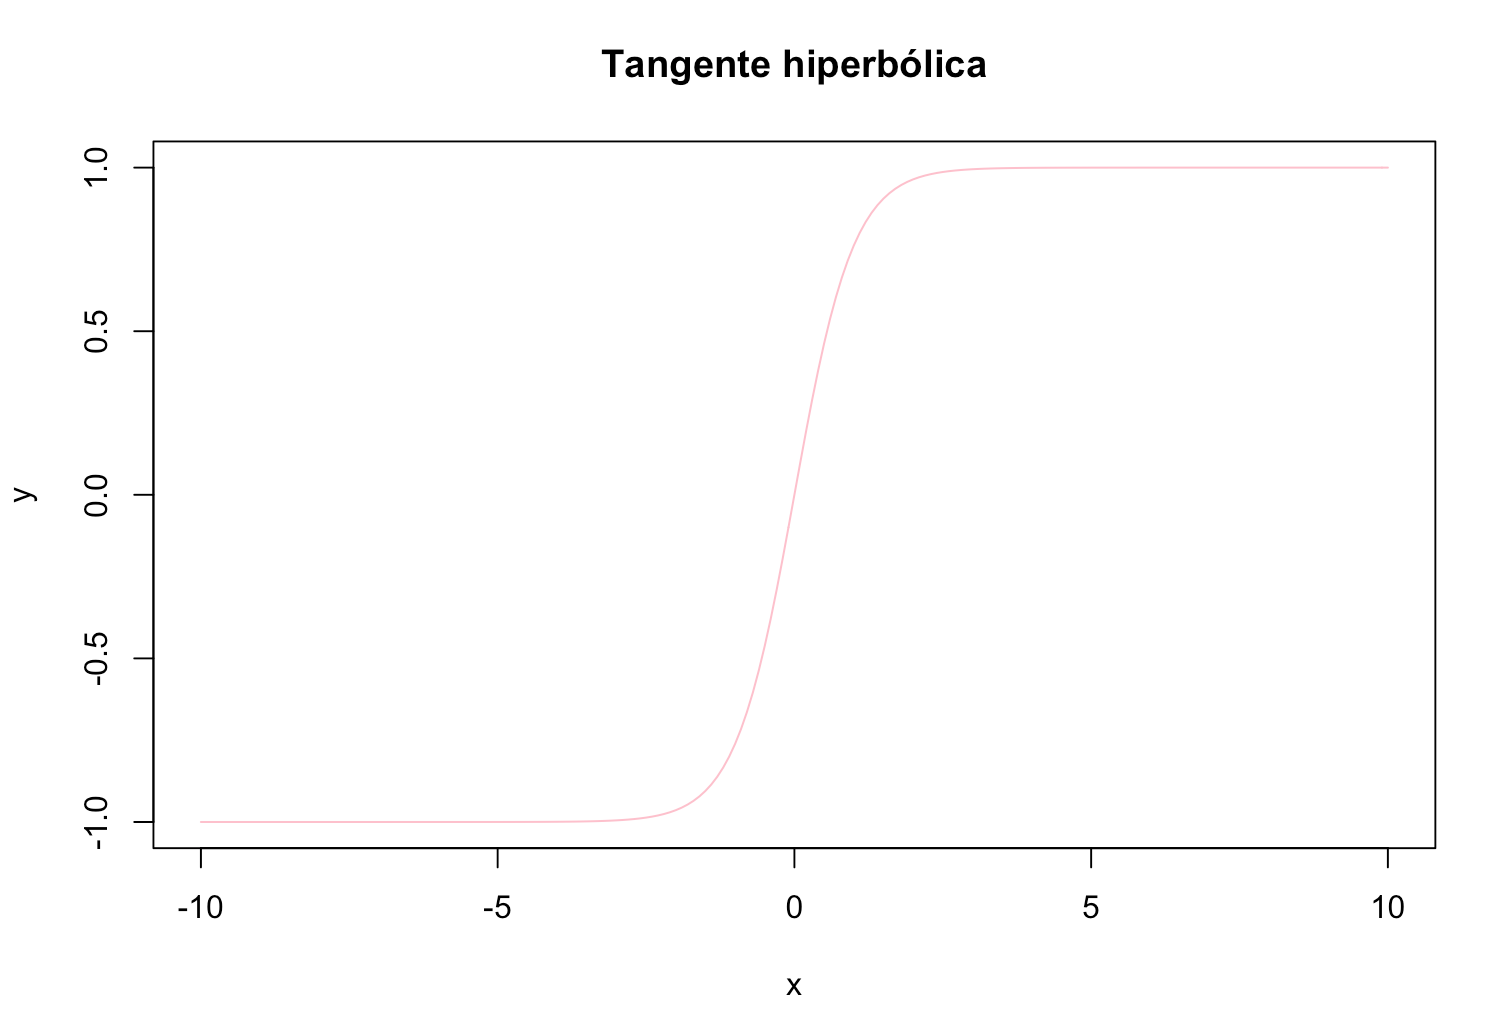
\includegraphics[width=0.8\linewidth]{imagenes/tanh}
		\caption{Gráfica de la tangente hiperbólica.}
		\label{fig:tanh}
	\end{figure}
	
	Ambas funciones de activación están relacionadas mediante la fórmula $\tanh(z) = 2 \sigma(2z) - 1$.
	
	
